% !TeX spellcheck = en_US
%\label{section:metodeLipide}

%In the previous chapter, the method of using a sacrificial layer to detach ice is discussed. For this, lipids need to be dissolved at cryogenic temperatures. As not every lipid is dissoluble in all solvents, an experiment is conducted to obtain solvents at room temperature. Then the best solvents are tested at cryogenic temperatures.

%TODO QUESTION: Does a Solvent exist which is able to dissolve a sacrificial layer of lipids?

Lipids are chosen because they possess a hydrophobic and hydrophilic part. They can hold an ice layer onto a hydrophobic sample holder without any other modifications which could increase adhesion. Also, lipids are dissolvable in common solvents which are liquid at cryogenic temperatures. Therefore, dissolving lipids at cryogenic temperatures to separate the ice layer would be a practical and gentle way to separate the ice layer. To test this theory, a strong enough solubility of Lipids at cryogenic temperatures must be proven first. 

Solubility is temperature dependent. The process of dissolving a solute in a solvent can be virtually broken down into three steps: First, the structure of the solute must be broken up with energy. Second the structure of the solvent is broken up also using energy. Last, the solute and solvent are rearranged into a new structure which releases energy. Depending on the ratio of energy used by breaking the structure of solute and solvent and the energy released at rearranging, the process is more or less endo- or exothermic \cite{ZafirJaveed.}. Exothermic processes have higher solubility at low temperatures, while Endothermic processes have higher solubility at high temperatures \cite{Mortimer.2007}. 

A quick look at the chemical structure of lipids reveals that solving lipids is most likely endothermic. lipids ordered in layers are held together with van-der-vaals forces, hydrogen bondings and electrostatic bonds \cite{RWayneAlbers.1999}. This results in a very strong bond between lipids. Therefore, a high amount of energy is needed to break up the lipid layer structure. This makes a resulting endothermic dissolving process likely.

For dissolving lipids at cryogenic temperatures, exothermic processes are favorable. Still, exothermic processes release energy in form of heat, which can damage the ice layer when heated up too much. Therefore, a mostly neutral dissolving process is optimal. 

Additionally, some solvents tested are soluble in water. It is unknown whether the solvents could be solved or diffuse inside the ice layer at \SI{-140}{\degreeCelsius}. Therefore the ice layer could be changed in some undesired manner. if a sufficient solvent is found and the solvent is soluble in water, a potential change of the vitrified ice needs to be addressed.

Tests are conducted to find a solvent to dissolve a sacrificial layer out of lipids. Two consecutive solubility experiments are proposed. The first experiment is conducted at room temperature. the aim is to find solvents with high solubility at room temperature. the candidates with high solubility are then tested in the next experiment at cryogenic temperature. the aim is now to find solvents with also high solubility at cryogenic temperatures. The first experiment is conducted as there are only three baths available at cryogenic temperature. therefore the throughput for experiments is limited. All tests are conducted on lipid and parylene coated sample holders.

\section{Preparation of lipid coated slides}

Two different kind of lipids are used: DOPC and EGG-PC. DOPC is storaged as a powder. The DOPC powder is dissolved in Ethanol ($25\,\si{\milli\gram}/1\,\si{\milli\liter}$ lipid to solvent) for application. EGG-PC is shipped solved in chloroform in two different ratios: $25\,\si{\milli\gram}/1\,\si{\milli\liter}$ and $10\,\si{\milli\gram}/1\,\si{\milli\liter}$. The solution is shipped in vials.

The solution containing lipids is transferred into several small bottles. they are chosen over a big bottle because solution forms a lubricating film on the thread of the lid. This film prevents the lid from closing airtight. non airtight bottles lead to evaporation of the solvent over time, changing and destroying the solution inside. In the coating process, solution often drops onto the threads, making a bottle only usable in one coating session. By splitting the solution into multiple bottles, more slides can be covered by one batch of lipid containing solution.

%Each solvent is put in a separate bottle. The lipid coated slides are prepared as previously described. For each solvent, a slide is put in the corresponding bottle. After \SI{15}{\minute}, the slides are removed and examined. The results are documented in a list. When all streaks caused by the lipid layer disappeared, the solvent is tested in the next experiment.

% TODO schauen ob da noch was wichtiges steht: To apply Phospholipids, a slide is dipped into the solution containing the phospholipid. When the solvent evaporates, the lipids are binding to the surface of the slide, forming a layer with varying homogeneity. this layer is removable with the same solvents. If the ice layer is frozen onto the lipid layer, the lipids can be dissolved at cryogenic temperatures as a sacrificial layer to detach the ice. But to dissolve this layer, a high solubility at cryogenic temperatures is required. The ice layer on top is a barrier between solvent and solute, reducing the area where solvent and lipids are directly in contact to the outer edge of the sample. 

Solvents for dissolving the sacrificial layer are chosen based on availability, freezing point and safety. These solvents are readily available in the laboratory. Some are ordered before the test. All chosen solvent need to be save to use in a well ventilated room. The dissolving cannot be conducted under a extractor hood as too much space is taken up with the experiment. Also the solvent needs to stay liquid at around \SI{-140}{\degreeCelsius} to assure that the ice layer on top stays vitrified. The tested substances are 4-Methyl Pentene, 3-Methyl Pentene, 1-Pentene, Isopentane, 1-Propanol, Pentane and Ethanol. 

As not all solvents are liquid at \SI{-140}{\degreeCelsius} (Table \ref{table:SchmelztemperaturLösungsmittel}), they are tested at higher temperatures above their melting point. In addition they are tested as mixtures with other solvents with a lower melting point. Additionally liquid ethane is tested only at  \SI{-140}{\degreeCelsius}. Ethane is not tested at room temperature, as the boiling point of ethane is at \SI{-88.6}{\degreeCelsius} \cite{PubChem.29.08.2023}.

%The freezing point of tested solvents are not all below \SI{-140}{\degreeCelsius}] (Table \ref{table:SchmelztemperaturLösungsmittel}). Still, solvents with a high freezing point can be mixed with other solvents with lower freezing point to lower the freezing point of the mixture. Alternatively, the temperature can be raised over the freezing point, but this could risk the ice to loose the vitrified state.

\begin{table}[hbt!]
	\centering
	\begin{tabular}{|l|c|}
		\hline
		solvent & melting point in °C \\
		\hline
		\hline
		4-Methyl Pentene & -154 \\ 
		\hline
		3-Methyl Pentene & -154 \\
		\hline
		1-Pentene & -165 \\
		\hline
		Isopentane & -160 \\
		\hline
		1-Propanol & -126 \\
		\hline
		Pentane & -129 \\
		\hline
		Ethanol & -114 \\
		\hline
	\end{tabular}
	\caption{Melting Point in °C for tested solvents.}
	\label{table:SchmelztemperaturLösungsmittel}
\end{table}

The solubility of lipids is tested on coated sample holders without the ice layer. a round $\varnothing$\SI{5}{\milli\meter} cover glass is chosen as sample holder as cheap substitute. The cover glass is coated with a thin layer of parylene. The coated cover glass is dipped into lipid solution. Then the coated cover glass is dried, leaving behind a lipid layer on the parylene. After preparation, streaks are visible on the sample holder which indicate the presence of lipids forming an irregular lipid layer (fig. \ref{fig:streaksOnSampleHolder}). The prepared sample holders are then used in solubility experiments.

\begin{figure}[hbt!]
	\centering
	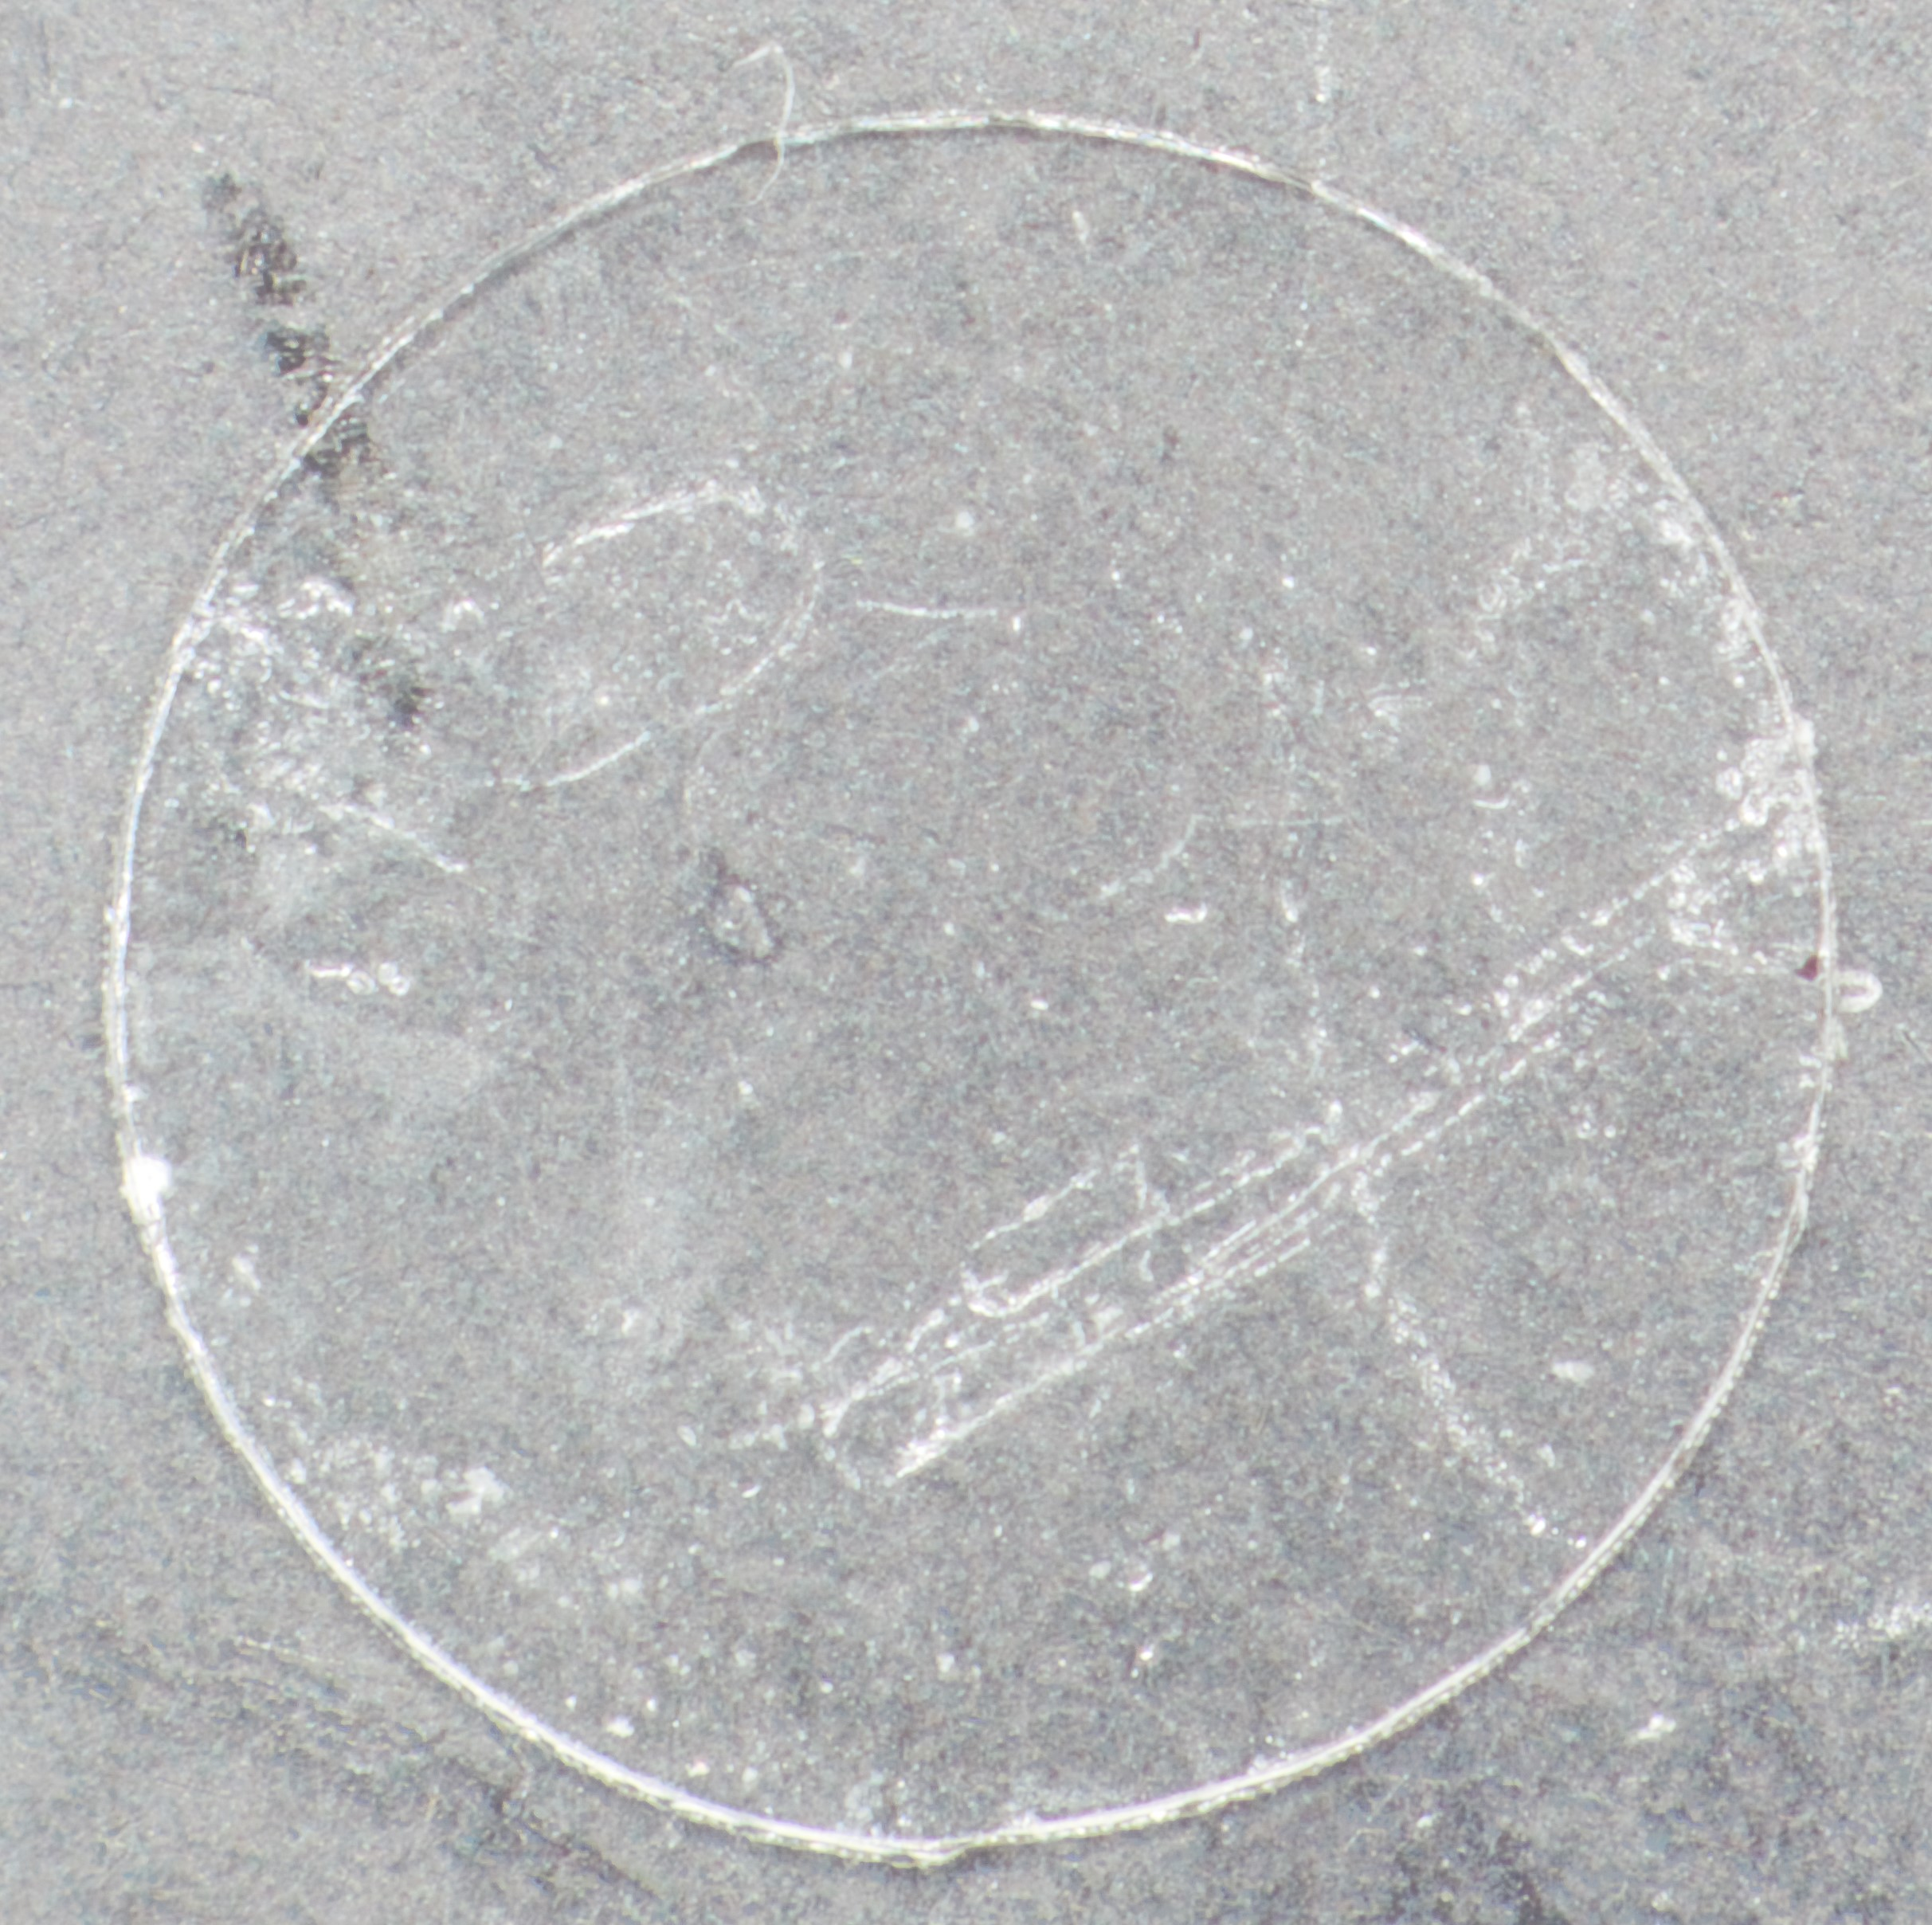
\includegraphics[width=7cm]{SlideWIthLipidStreaks.jpg}
	\caption{Example of a $\varnothing$\SI{5}{\milli\meter} cover glass with streaks of lipid residuals on the surface.}
	\label{fig:streaksOnSampleHolder}
\end{figure}

\subsection{at room temperature}

The solubility of lipids in different solvents are determined at room temperature first. For this experiment, the sample holders are prepared as described before. Then a first reference image was taken. The cover glass is given into a small container with the solvent candidate. After 15 minutes, the sample holder is removed and compared under the microscope with the reference picture. If streaks created from lipids are still as visible as before, the lipids are categorized as insoluble in this solvent. If the streaks partially disappeared and/or are less visible, the lipids are categorized as partially soluble in this solvent. Last if the streaks completely disappear, the lipids are assinged as soluble in the solvent (Table \ref{table:LoeslichkeitRaumtemperatur}).


\begin{table}[hbt!]
	\centering
	\begin{tabular}{|l|c|c|}
		\hline
		potential solvent & solubility EGG-PC & solubility DOPC \\
		\hline
		\hline
		4-Methyl Pentene & soluble & N/A  \\ 
		\hline
		3-Methyl Pentene & slightly soluble & insoluble \\
		\hline
		1-Pentene & insoluble & insoluble \\
		\hline
		Isopentane & soluble & slightly soluble\\
		\hline
		1-Propanol & soluble & soluble\\
		\hline
		Pentane & soluble & insoluble\\
		\hline
		Ethanol & N/A & soluble\\
		\hline
	\end{tabular}
	\caption{Result of solubility tests at room temperature. Soluble indicates solvents which are able to visibly solve all lipids off a cover glass. slightly soluble indicates solutions which are able to solve lipids with residuals. Insoluble indicates no visible removal of tested lipid.}
	\label{table:LoeslichkeitRaumtemperatur}
\end{table}

This experiment shows that each three different solvent exist for EGG-PC and DOPC with high solubility (Table \ref{table:LoeslichkeitRaumtemperatur}). Following these results, solvents categorized with "soluble" are tested regarding solubility at temperatures of \SI{-140}{\degreeCelsius}. 

\subsection{at cryogenic temperature}
\label{chapter:meltingtemp}

The experiment is conducted at \SI{-140}{\degreeCelsius}. The solvents are given in liquid nitrogen cooled baths, which are regulated to the desired temperature. A slide is given into the cold solvent for \SI{15}{\minute}. Then the slide is examined for leftover streaks as before.

In the experiment, no tested solvent was able to completely solve lipids at \SI{-140}{\degreeCelsius} and within \SI{15}{\minute} (Table \ref{table:Cryoloeslichkeit}). Also streaks of applied lipids did not only stay partially behind, but also new streaks appear on the glass slides. This means that some lipids redistributed on the same glass slide.

\begin{table}[hbt!]
	\begin{subtable}{\linewidth}
		\centering
		\begin{tabular}{|l|l|}
			\hline
			Solvent & Result \\
			\hline
			\hline
			Pentane & soluble at \SI{-125}{\degreeCelsius} \\
			\hline
			4-methyl pentene & insoluble \\
			\hline
			\makecell[l]{1:1 volume ratio\\ HFE to 1-Propanol} & \makecell[l]{not mixable,\\ slightly soluble}\\
			\hline
			Liquid ethane & insoluble\\
			\hline
		\end{tabular}
		\caption{EGG-PC}
		\label{table:EGG-PCCryoloeslichkeit}
	\end{subtable}
	\begin{subtable}{\linewidth}
		\centering
		\begin{tabular}{|l|l|}
			\hline
			Solvent & Result \\
			\hline
			\hline
			\makecell[l]{1:4 volume ratio\\ 1:2 molar ratio\\ Ethanol to Isopentane} & slightly soluble\\
			\hline
			\makecell[l]{1:2 volume ratio\\ 1:1 molar ratio\\ 1-Propanol to Isopentane} & insoluble \\
			\hline
			Isopentane & slightly soluble\\
			\hline
			1-Propanol & \makecell[l]{at \SI{-130}{\degreeCelsius}\\ slightly soluble}\\
			\hline
			Liquid ethane & insoluble \\
			\hline
		\end{tabular}
		\caption{DOPC}
		\label{table:DOPCCryoloeslichkeit}
	\end{subtable}
	\caption{ in \ref{table:EGG-PCCryoloeslichkeit} for EGG-PC, no sufficient solubility at -140°C was found. In \ref{table:EGG-PCCryoloeslichkeit}, DOPC was tested but also no proper solution was found.}
	\label{table:Cryoloeslichkeit}
\end{table}

Using solvents to remove a sacrificial layer, a high solubility is required. In practice, the sacrificial layer is completely covered by the ice layer except the edges. Therefore area of contact with the solvent is small, slowing the process considerably. Additionally, as the ice layer needs to stay vitrified. The temperature cannot be raised over \SI{-140}{\degreeCelsius} to speed up the process.

The solving process of lipids proves to be endothermic. This means that heat is needed to solve lipids, so cold temperature heavily decrease solubility. This effect was observed over the last experiments by all solvents to varying degree. It can be assumed that the majority of solvent lipids mixtures are endothermic which is very disadvantageous for finding a potential solvent lipid candidate. Strongly exothermic solvents could heat up the ice enough to crystallize the ice. So weakly exothermic solvents would be optimal for this task.